\documentclass{tmr}

\usepackage{graphicx}

\renewcommand{\thetable}{\arabic{table}}

\usepackage{prettyref}
\newrefformat{fig}{Figure~\ref{#1}}
\newrefformat{tab}{Table~\ref{#1}}

\newcommand{\italic}[1]{\textit{#1}}

\title{Generalized Algebraic Data Types in Haskell}
\author{Anton Dergunov\email{anton.dergunov@gmail.com}}

\begin{document}

\begin{introduction}

Generalized algebraic data types (GADTs) are a feature of functional programming languages which generalize ordinary algebraic data types by permitting value constructors to return specific types. This article is a tutorial about GADTs in Haskell programming language as they are implemented by the Glasgow Haskell Compiler (GHC) as a language extension. GADTs are widely used in practice: for domain-specific embedded languages, for generic programming, for ensuring program correctness and in other cases. The article describes these use cases with small GADT programs and also describes usage of GADTs in Yampa, a Haskell library.

\end{introduction}

\section{Introduction}

The usage of type systems is recognized as the most popular and best established lightweight formal method for ensuring that software behaves correctly~\cite{pierce_book}. It is used for detecting program errors, for documentation, to enforce abstraction and in other cases. The study of type systems is an active research area and Haskell is considered to be a kind of laboratory in which type-system extensions are designed, implemented and applied~\cite{haskell_history}. This article is a tutorial about one such extension -- generalized algebraic data types (GADTs). The theoretical foundation for GADTs is the notion of dependent types which is extensively described in literature on computer science and logic~\cite{pierce_book}.

GADTs are very useful in practice. Several examples of GADTs usage are described in this article. But these examples are not new. They were taken from many resources~\cite{fun_with_phantom_types,replib,singletons,okasaki_red_black_trees,weirich_dependently_typed,finally_tagless,yampa_gadts} and many examples are already a part of Haskell folklore.

The contribution of this article is presenting a concise introductory-level tutorial on the concept and popular use cases of GADTs. The following use cases were described in this article:

\begin{itemize}
\item domain-specific embedded languages;
\item generic programming;
\item ensuring program correctness.
\end{itemize}

We describe why type signatures are required for functions involving GADTs; the usage of GADTs in Yampa, a domain-specific language for functional reactive programming; an alternative implementation of one of the examples without GADTs usage. Additionally, several other Haskell extensions are covered in passing where necessary, such as type families and data kinds.

All examples in this article were tested with Glasgow Haskell Compiler, version 7.4.1.

\section{GADTs in a Nutshell}
\label{sec:nutshell}

\italic{Algebraic data types} (ADTs) are declared using the data keyword:

\begin{Verbatim}
data Test a = TI Int | TS String a
\end{Verbatim}

In the example above \verb}Test} is called a \italic{type constructor}. \verb|TI| and \verb|TS| are \italic{value constructors}. If a type has more than one value constructor, they are called \italic{alternatives}: one can use any of these alternatives to create a value of that type. Each alternative can specify zero or more components. For example, \verb|TS| specifies two components: one of them has type \verb|String| and another one -- type \verb|a|.

We can construct values of this type this way:

\begin{Verbatim}
ghci> let a = TI 10
ghci> :t a
a :: Test a
ghci> let b = TS "test" 'c'
ghci> :t b
b :: Test Char
\end{Verbatim}

Value constructors of the type \verb|Test| have the following types:

\begin{Verbatim}
ghci> :t TI
TI :: Int -> Test a
ghci> :t TS
TS :: String -> a -> Test a
\end{Verbatim}

Using GADT syntax we can define the \verb|Test| data type as:

\begin{Verbatim}
data Test a where
    TI :: Int -> Test a
    TS :: String -> a -> Test a
\end{Verbatim}

The GADTs feature is a Haskell language extension. Just like other extensions it can be enabled in GHC by:

\begin{longenum}

\item Using command line option \verb|-XGADTs|.

\item Using \verb|LANGUAGE| pragma in source files. This is the recommended way, because it enables this language extension per-file. This pragma must precede the module keyword in the source file and contain the following:
\begin{Verbatim}
{-# LANGUAGE GADTs #-}
\end{Verbatim}

\end{longenum}

The power of GADTs is not about syntax. In fact, \italic{the single idea of GADTs is to allow arbitrary return types of value constructors}. In this way they generalize ordinary algebraic data types. Of course, this return type must still be an instance of the more general data type that is defined. We can turn the \verb|Test| data type into a full-power GADT for example this way:

\begin{Verbatim}
data Test a where
    TI :: Int -> Test Int
    TS :: String -> a -> Test a
\end{Verbatim}

We have modified the \verb|TI| value constructor to return value of type \verb|Test Int| and we can test this:

\begin{Verbatim}
ghci> :t TI 10
TI 10 :: Test Int
\end{Verbatim}

While creating a values with the \verb|TI| results in a value of type \verb|Test Int|, the converse holds too: when a pattern-match succeeds on the \verb|TI| constructor in the example below, we can now conclude that the type of \verb|a| is \verb|Int|. That is to say, pattern matching causes type refinement, which is the key feature of GADTs.

\begin{Verbatim}
f :: Test a -> a
f (TI i) = i + 10
\end{Verbatim}

Examples in the following sections show some practical applications of GADTs.

\section{Expression Evaluator}
\label{sec:expression_evaluator}

This section introduces GADTs with the canonical example of an expression evaluator. At first, we attempt to implement it using ordinary algebraic data types. But as we will see, GADTs allow a more elegant implementation of the evaluator.

We start with the following type of expressions involving addition of integers:

\begin{Verbatim}
data IntExpr = IntVal Int
             | AddInt IntExpr IntExpr
\end{Verbatim}

\verb|IntVal| value constructor is used to wrap integer literal and \verb|AddInt| is used to represent an addition of two integer expressions. An example of such expression is:

\begin{Verbatim}
ghci> :t AddInt (IntVal 5) (IntVal 7)
AddInt (IntVal 5) (IntVal 7) :: IntExpr
\end{Verbatim}

Evaluation function for such expressions is easy to write:

\begin{Verbatim}
evaluate :: IntExpr -> Int
evaluate e = case e of
    IntVal i     -> i
    AddInt e1 e2 -> evaluate e1 + evaluate e2
\end{Verbatim}

Now we extend the type of expressions to support boolean values and add some operations on them:

\begin{Verbatim}
data ExtExpr = IntVal Int
             | BoolVal Bool
             | AddInt ExtExpr ExtExpr
             | IsZero ExtExpr
\end{Verbatim}

\verb|BoolVal| value constructor wraps Boolean literal. \verb|IsZero| is a unary function that takes an integer and returns a Boolean value. We immediately notice a problem with this type: it is possible to write incorrect expressions that type checker will accept. For example:

\begin{Verbatim}
ghci> :t IsZero (BoolVal True)
IsZero (BoolVal True) :: ExtExpr
ghci> :t AddInt (IntVal 5) (BoolVal True)
AddInt (IntVal 5) (BoolVal True) :: ExtExpr
\end{Verbatim}

Evaluation function for such expressions is also tricky. The result of evaluation can be either an integer or a Boolean value. The type \verb|ExtExpr| is not parametrized by return value type, so we have to use type \verb|Either Int Bool|. Furthermore, evaluation will fail if the input expression is incorrect, so we have to use type \verb|Maybe|. Finally, the type signature of \verb|evaluate| is the following:

\begin{Verbatim}
evaluate :: ExtExpr -> Maybe (Either Int Bool)
\end{Verbatim}

Implementing this function is complicated. For example, processing \verb|AddInt| requires usage of a nested \verb|case|:

\begin{Verbatim}
evaluate e = case e of
    AddInt e1 e2 -> case (evaluate e1, evaluate e2) of
        (Just (Left i1), Just (Left i2)) -> Just $ Left $ i1 + i2
        _ -> fail "AddInt takes two integers"
\end{Verbatim}

The conclusion is that we need to represent expressions using values of types parametrized by expression return value type. \italic{Phantom type} is a parametrized type whose parameters do not appear on the right-hand side of its definition. One can use them this way:

\begin{Verbatim}
data PhantomExpr t = IntVal Int
                   | BoolVal Bool
                   | AddInt (PhantomExpr Int) (PhantomExpr Int)
                   | IsZero (PhantomExpr Int)
\end{Verbatim}

Type \verb|t| in this type corresponds to the expression return value type. For example, integer expression has type \verb|PhantomExpr Int|. But this type definition alone is still not helpful, because it is still possible to write incorrect expressions that type checker will accept:

\begin{Verbatim}
ghci> :t IsZero (BoolVal True)
IsZero (BoolVal True) :: PhantomExpr t
\end{Verbatim}

The trick is to wrap value constructors with corresponding functions:

\begin{Verbatim}
intVal :: Int -> PhantomExpr Int
intVal = IntVal
boolVal :: Bool -> PhantomExpr Bool
boolVal = BoolVal
isZero :: PhantomExpr Int -> PhantomExpr Bool
isZero = IsZero
\end{Verbatim}

And now bad expressions are rejected by type checker:

\begin{Verbatim}
ghci> :t isZero (boolVal True)
Couldn't match expected type `Int' with actual type `Bool'...
ghci> :t isZero (intVal 5)
isZero (intVal 5) :: PhantomExpr Bool
\end{Verbatim}

Ideally, we want the following type signature for \verb|evaluate| method:

\begin{Verbatim}
evaluate :: PhantomExpr t -> t
\end{Verbatim}

But we can't define such function. For example, the following line produces error ``\verb|Couldn't match type `t' with `Int'|'':

\begin{Verbatim}
evaluate (IntVal i) = i
\end{Verbatim}

The reason of this error is that return type of value constructor \verb|IntVal| is \verb|Phantom t| and \verb|t| can be refined to any type. For example:

\begin{Verbatim}
ghci> :t IntVal 5 :: PhantomExpr Bool
IntVal 5 :: PhantomExpr Bool :: PhantomExpr Bool
\end{Verbatim}

What is really needed here is to specify type signature of value constructors exactly. In this case pattern matching in \verb|evaluate| would cause type refinement for \verb|IntVal|. And this is exactly what GADTs do.

As described in the previous section, GADTs use a different syntax than ordinary algebraic data types. In fact, value constructors specified by the data type \verb|PhantomExpr| can be written as the following functions:

\begin{Verbatim}
IntVal  :: Int -> PhantomExpr t
BoolVal :: Bool -> PhantomExpr t
AddInt  :: PhantomExpr Int -> PhantomExpr Int -> PhantomExpr t
IsZero  :: PhantomExpr Int -> PhantomExpr t
\end{Verbatim}

Using GADT syntax, the data type \verb|PhantomExpr| type can be declared this way:

\begin{Verbatim}
data PhantomExpr t where
    IntVal  :: Int -> PhantomExpr t
    BoolVal :: Bool -> PhantomExpr t
    AddInt  :: PhantomExpr Int -> PhantomExpr Int -> PhantomExpr t
    IsZero  :: PhantomExpr Int -> PhantomExpr t
\end{Verbatim}

All value constructors have \verb|PhantomExpr t| as their return type. As noted in the previous section, the distinctive feature of GADTs is the ability to return specific types in value constructors, for example \verb|PhantomExpr Int|. The expression language can be written with GADTs in this fashion:

\begin{Verbatim}
data Expr t where
    IntVal  :: Int -> Expr Int
    BoolVal :: Bool -> Expr Bool
    AddInt  :: Expr Int -> Expr Int -> Expr Int
    IsZero  :: Expr Int -> Expr Bool
    If      :: Expr Bool -> Expr t -> Expr t -> Expr t
\end{Verbatim}

Note that value constructors of this data type have specific return types. Now bad expressions are rejected by the type checker:

\begin{Verbatim}
ghci> :t IsZero (BoolVal True)
Couldn't match expected type `Int' with actual type `Bool'...
ghci> :t IsZero (IntVal 5)
IsZero (IntVal 5) :: Expr Bool
\end{Verbatim}

Note that the type of value \verb|IsZero (IntVal 5)| is specific: \verb|Expr Bool|.

GADTs allow to write well-defined \verb|evaluate| function:

\begin{Verbatim}
evaluate :: Expr t -> t
evaluate (IntVal i)     = i
evaluate (BoolVal b)    = b
evaluate (AddInt e1 e2) = evaluate e1 + evaluate e2
evaluate (IsZero e)     = evaluate e == 0
evaluate (If e1 e2 e3)  = if evaluate e1 then
    evaluate e2 else evaluate e3
\end{Verbatim}

Pattern matching causes type refinement: the right-hand side of the following expression \verb|i| has type \verb|Int|:

\begin{Verbatim}
evaluate :: Expr t -> t
evaluate (IntVal i) = ...
\end{Verbatim}

The type of \verb|AddInt e1 e2| expression is \verb|Expr Int| and the types of \verb|e1| and \verb|e2| must also be \verb|Expr Int|, so we can evaluate recursively the individual expressions and then return the sum (value of type \verb|Int|).

At the end of this article, we describe one more implementation of expression evaluator.

\section{Generic Programming with GADTs}
\label{sec:generic_programming}

In datatype-generic programming, functions take a type as an argument and change behavior depending on the structure of this type. There are several approaches to such kind of generic programming in Haskell. A paper by Hinze et al.~\cite{generic_programming} provides an overview of these approaches. In this section, we present an approach which uses GADTs. Ideas for this section were taken from another paper by Hinze at al.~\cite{fun_with_phantom_types}.

Suppose we would like to write a function to encode data in binary form. This function must be able to work with values of several types. Functions like this one can be implemented using type classes. However, GADTs offer an interesting alternative.

First we need to declare a \italic{representation type}~\cite{replib}, a type whose values represent types:

\begin{Verbatim}
data Type t where
    TInt  :: Type Int
    TChar :: Type Char
    TList :: Type t -> Type [t]
\end{Verbatim}

This is GADT with value constructors that create a representation of the corresponding type. For example:

\begin{Verbatim}
ghci> let a = TInt
ghci> :t a
a :: Type Int
ghci> let b = TList TInt
ghci> :t b
b :: Type [Int]
\end{Verbatim}

\verb|String| type is defined in Haskell as a list of \verb|Char| elements, so we can define a value constructor for string type representation this way:

\begin{Verbatim}
tString :: Type String
tString = TList TChar
\end{Verbatim}

The output of the encoding function is a list of bits where bits are represented using:

\begin{Verbatim}
data Bit = F | T deriving(Show)
\end{Verbatim}

The encoding function takes a representation of the type, the value of this type and returns a list of bits.

\begin{Verbatim}
encode :: Type t -> t -> [Bit]
encode TInt i = encodeInt i
encode TChar c = encodeChar c
encode (TList _) [] = F : []
encode (TList t) (x : xs) = T :
    (encode t x) ++ encode (TList t) xs
\end{Verbatim}

We can test this function:

\begin{Verbatim}
ghci> encode TInt 333
[T,F,T,...,F,F,F]
ghci> encode (TList TInt) [1,2,3]
[T,T,F,...,F,F,F]
ghci> encode tString "test"
[T,F,F,...,F,F,F]
\end{Verbatim}

If we pair the representation type and the value together, we get a \italic{universal data type}, the type \verb|Dynamic| (this code requires using \verb|ExistentialQuantification| extension):

\begin{Verbatim}
data Dynamic = forall t. Dyn (Type t) t
\end{Verbatim}

Above we have defined an \italic{existential data type} which can also be represented as a GADT:

\begin{Verbatim}
data Dynamic where
    Dyn :: Type t -> t -> Dynamic
\end{Verbatim}

Now we can declare a variant of \verb|encode| function which gets a \verb|Dynamic| type value as input:

\begin{Verbatim}
encode' :: Dynamic -> [Bit]
encode' (Dyn t v) = encode t v
\end{Verbatim}

The following session illustrates the usage of this type:

\begin{Verbatim}
ghci> let c = Dyn (TList TInt) [5,4,3]
ghci> :t c
c :: Dynamic
ghci> encode' c
[T,T,F,...,F,F,F]
\end{Verbatim}

We can now define heterogeneous lists using the \verb|Dynamic| type:

\begin{Verbatim}
ghci> let d = [Dyn TInt 10, Dyn TString "test"]
ghci> :t d
d :: [Dynamic]
\end{Verbatim}

However, we can't make this list a \verb|Dynamic| value itself. To fix this problem, we need to extend the representation type, adding a value constructor for the \verb|Dynamic| data type.

\begin{Verbatim}
data Type t where
    ...
    TDyn :: Type Dynamic
\end{Verbatim}

We also need to update \verb|encode| function to handle the \verb|Dynamic| data type:

\begin{Verbatim}
encode :: Type t -> t -> [Bit]
...
encode TDyn (Dyn t v) = encode t v
\end{Verbatim}

Now we can represent a list of \verb|Dynamic| values as a \verb|Dynamic| value itself and encode it:

\begin{Verbatim}
ghci> let d = [Dyn TInt 10, Dyn tString "test"]
ghci> :t d
d :: [Dynamic]
ghci> let e = Dyn (TList TDyn) d
ghci> :t e
e :: Dynamic
ghic> encode' e
[T,F,T,...,F,F,F]
\end{Verbatim}

The \verb|Dynamic| data type is useful for communication with the environment when the actual type of the data is not known in advance. In this case a type cast is required to get useful data. A simple way to implement a type cast from \verb|Dynamic| data type to an integer is the following:

\begin{Verbatim}
castInt :: Dynamic -> Maybe Int
castInt (Dyn TInt i) = Just i
castInt (Dyn _ _) = Nothing
\end{Verbatim}

There is a more generic solution~\cite{fun_with_phantom_types} for this problem that works for all types, not just integer, but it is out of scope for this article.

While the presented approach is an important use case of GADTs, the disadvantage of this approach is that we have to extend the representation type whenever we define a new data type.

\section{Proving Correctness of List Operations}
\label{sec:list_operations}

An important role of type systems is to ensure that data is manipulated in appropriate ways (for example, to ensure we pass a list to \verb|head| function). But types can be used to express more sophisticated properties. For example, we can define a type of lists of a particular length and then define a \verb|headSafe| function that only accepts non-empty lists. The idea described in this section is to use types to express correctness properties and then use type checker of the programming language to ensure that we can express only those programs that have the desired properties. This idea was developed in $\Omega$mega system~\cite{curry_howard,omega}. In this section, we use GADTs in the Haskell programming language to prove the correctness of list operations; in the next section, we describe how to use GADTs to prove correctness of the insertion operation in red-black trees.

Lists can be represented using the following algebraic data type:

\begin{Verbatim}
data List t = Nil | Cons t (List t)
\end{Verbatim}

or using GADT syntax as:

\begin{Verbatim}
data List t where
    Nil :: List t
    Cons :: t -> List t -> List t
\end{Verbatim}

Now \verb|head| function can be implemented this way:

\begin{Verbatim}
listHead :: List t -> t
listHead (Cons a _) = a
listHead Nil = error "list is empty"
\end{Verbatim}

The disadvantage of this function is that it can fail: it fails when a list is empty and succeeds otherwise. To address this problem we define a type of non-empty lists. First we define two empty data types (this requires \verb|EmptyDataDecls| extension):

\begin{Verbatim}
data Empty
data NonEmpty
\end{Verbatim}

Now we define a safe list GADT:

\begin{Verbatim}
data SafeList t f where
    Nil :: SafeList t Empty
    Cons :: t -> SafeList t f -> SafeList t NonEmpty
\end{Verbatim}

Parameter \verb|f| takes type \verb|Empty| when the list is empty and \verb|NonEmpty| otherwise. The function \verb|headSafe| is a safe version of \verb|listHead| function that only accepts non-empty lists as parameter.

\begin{Verbatim}
headSafe :: SafeList t NonEmpty -> t
headSafe (Cons t _) = t
\end{Verbatim}

For example:

\begin{Verbatim}
ghci> headSafe Nil
Couldn't match expected type `NonEmpty' with actual type `Empty'
ghci> headSafe $ Cons 1 $ Cons 2 $ Cons 3 Nil
1
\end{Verbatim}

However, the implementation of a function to create a list containing an element repeated a given number of times using \verb|SafeList| data type is problematic: it is not possible to determine return value type of this function.

\begin{Verbatim}
repeatElem :: a -> Int -> SafeList a ???
repeatElem a 0 = Nil
repeatElem a n = Cons a (repeatElem a (n-1))
\end{Verbatim}

The problem is that empty and non-empty lists have completely different types. To fix this problem we can slightly relax \verb|Cons| value constructor:

\begin{Verbatim}
data SafeList t f where
    Nil :: SafeList t Empty
    Cons :: t -> SafeList t f -> SafeList t f'
\end{Verbatim}

Now \verb|SafeList t Empty| is a type of possibly empty lists, for example:

\begin{Verbatim}
ghci> :t Nil
Nil :: SafeList t Empty
ghci> :t Cons 'a' Nil
Cons 'a' Nil :: SafeList Char f'
ghci> :t Cons 'a' Nil :: SafeList Char Empty
Cons 'a' Nil :: SafeList Char Empty :: SafeList Char Empty
ghci> :t Cons 'a' Nil :: SafeList Char NonEmpty
Cons 'a' Nil :: SafeList Char NonEmpty :: SafeList Char NonEmpty
\end{Verbatim}

And we can define \verb|repeatElem| as a function returning possibly empty lists:

\begin{Verbatim}
repeatElem :: a -> Int -> SafeList a Empty
repeatElem a 0 = Nil
repeatElem a n = Cons a (repeatElem a (n-1))
\end{Verbatim}

It's worth noting that with the current data type definition, a term \verb|Cons 'a' Nil| can even be given the type \verb|SafeList Char Int|. To fix this problem, we need to somehow give the \verb|Empty| and \verb|NonEmpty| types the same kind. This is discussed later for \verb|Nat| data type.

Regardless, \verb|SafeList| data type does not have enough static information to prove stronger list length invariants for many list functions. For example, for the concatenation function we need to show that length of the concatenated list is a sum of source lists lengths. It is not enough to just know if a list is empty or not: we need to encode the length of a list in its type.

The classical way to encode numbers at the type level is Peano numbers:

\begin{Verbatim}
data Zero
data Succ n
\end{Verbatim}

Zero is encoded as \verb|Zero|, one -- as \verb|Succ Zero|, two -- as \verb|Succ (Succ Zero)| and so on. Now the list data type is defined as:

\begin{Verbatim}
data List a n where
    Nil :: List a Zero
    Cons :: a -> List a n -> List a (Succ n)
\end{Verbatim}

Function \verb|headSafe| can be defined as:

\begin{Verbatim}
headSafe :: List t (Succ n) -> t
headSafe (Cons t _) = t 
\end{Verbatim}

We can also show that the safe map function does not change the length of a list:

\begin{Verbatim}
mapSafe :: (a -> b) -> List a n -> List b n
mapSafe _ Nil = Nil
mapSafe f (Cons x xs) = Cons (f x) (mapSafe f xs) 
\end{Verbatim}

To implement the concatenation function, we need a type-level function for addition of Peano numbers. A natural way to implement such function is to use \italic{type families} (which in context of this tutorial can be understood as type-level functions). First, we need to declare type family \verb|Plus| (this requires \verb|TypeFamilies| extension):

\begin{Verbatim}
type family Plus a b
\end{Verbatim}

Then, we need to declare type instances that implement addition of Peano numbers by induction:

\begin{Verbatim}
type instance Plus Zero n = n
type instance Plus (Succ m) n = Succ (Plus m n)
\end{Verbatim}

The type family \verb|Plus| that we have just defined can be used in the concatenation function signature:

\begin{Verbatim}
concatenate :: List a m -> List a n -> List a (Plus m n)
concatenate Nil ys = ys
concatenate (Cons x xs) ys = Cons x (concatenate xs ys)
\end{Verbatim}

As mentioned previously, \verb|Succ| has a type parameter of kind \verb|*|, so it possible to write nonsensical terms like \verb|Succ Int| which will be accepted by the type checker. This problem can be addressed using a new \italic{kind}. Just as types classify values, kinds classify types. We can declare the following data type:

\begin{Verbatim}
data Nat = Zero | Succ Nat
\end{Verbatim}

\begin{figure}
\centering
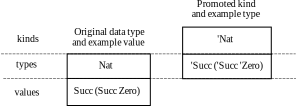
\includegraphics{promotion}
\vspace{5pt}
\caption{Promotion of a data type to a kind.}
\label{fig:promotion}
\end{figure}

Here \verb|Nat| is a type; \verb|Zero| and \verb|Succ| are value constructors. But due to promotion~\cite{promotion} \verb|Nat| also becomes a kind; \verb|Zero| and \verb|Succ| also become types (see \prettyref{fig:promotion}). Where necessary, a quote must be used to resolve ambiguity. For example, \verb|'Succ| refers to a type, not a value constructor. So, type-level representation of the number two can be written as:

\begin{Verbatim}
type T = 'Succ ('Succ 'Zero)
\end{Verbatim}

Quotes can be omitted in this case, because there is no ambiguity:

\begin{Verbatim}
type T2 = Succ (Succ Zero)
\end{Verbatim}

As a result, type checker now rejects wrong terms like \verb|Succ Int|.

The definition of the list data type can also be improved now to clearly specify that the type of its second parameter has kind \verb|Nat| (this requires \verb|DataKinds| extension):

\begin{Verbatim}
data List a (n::Nat) where
    Nil :: List a 'Zero
    Cons :: a -> List a n -> List a ('Succ n)
\end{Verbatim}

After the changes that we have made to the definition of the \verb|List| data type, the implementation of the \verb|repeatElem| function becomes more involved, because now we can't yet write its return type:

\begin{Verbatim}
repeatElem :: a -> Int -> List a ???
repeatElem a 0 = Nil
repeatElem a n = Cons a (repeatElem a (n-1))
\end{Verbatim}

On the one hand, the count parameter must be passed as a value to populate the list at run-time. On the other hand, we need a type-level representation of the same number for \verb|List| type. Haskell enforces a phase separation between run-time values and compile-time types. This causes a problem with the type signature of the function \verb|repeatElem|: there is no direct way to specify a type-level representation of list's count in the return value type of the function which will match the count passed in as a value.

The solution to this puzzle is the use of \italic{singleton types}. Singleton types are types that contain only one value (except, of course, the $\bot$ value, which is a member of every type in Haskell).

The singleton for Peano numbers type can be expressed using the following GADT:

\begin{Verbatim}
data NatSing (n::Nat) where
    ZeroSing :: NatSing 'Zero
    SuccSing :: NatSing n -> NatSing ('Succ n)
\end{Verbatim}

\begin{figure}
\centering
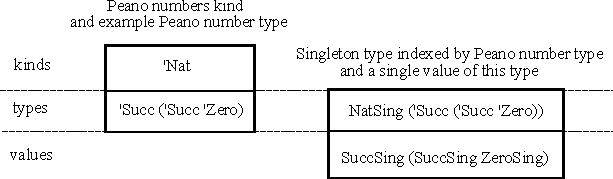
\includegraphics{singleton}
\vspace{5pt}
\caption{Singleton type for Peano numbers.}
\label{fig:singleton}
\end{figure}

The constructors of the singleton \verb|NatSing| mirror those of the kind \verb|Nat|. As a result, every type of kind \verb|Nat| corresponds to exactly one value (except $\bot$ value) of the singleton data type where parameter \verb|n| has exactly this type (see \prettyref{fig:singleton}). For example:

\begin{Verbatim}
ghci> :t ZeroSing
ZeroSing :: NatSing 'Zero
ghci> :t SuccSing $ SuccSing ZeroSing
SuccSing $ SuccSing ZeroSing :: NatSing ('Succ ('Succ 'Zero))
\end{Verbatim}

Now function \verb|repeatElem| can be defined this way:

\begin{Verbatim}
repeatElem :: a -> NatSing n -> List a n
repeatElem _ ZeroSing     = Nil
repeatElem x (SuccSing n) = Cons x (repeatElem x n)
\end{Verbatim}

In a function returning an element by index in the list we need to make sure that the index does not exceed the list length. This requires a type-level function to compute whether one number is less than the other. We define the following type family and instances (the \verb|TypeOperators| extension is required to be able to define \verb|:<| operation for types):

\begin{Verbatim}
type family (m::Nat) :< (n::Nat) :: Bool
type instance m         :< 'Zero     = 'False
type instance 'Zero     :< ('Succ n) = 'True
type instance ('Succ m) :< ('Succ n) = m :< n
\end{Verbatim}

This type-level function is implemented using induction. It returns promoted type \verb|'True| of kind \verb|Bool| when first number is less than the second one.

Now the function can be defined this way:

\begin{Verbatim}
nthElem :: (n :< m) ~ 'True => List a m -> NatSing n -> a
nthElem (Cons x _)  ZeroSing     = x
nthElem (Cons _ xs) (SuccSing n) = nthElem xs n
\end{Verbatim}

The tilde operation is an \italic{equality constraint}. It asserts that two types are the same in the context. Thus, is it only possible to use this function when the index does not exceed the list length.

We have shown that GADTs provide a way to use Haskell type checker to verify correctness of list operations. To do this, we need to specify necessary properties in the data type. The set of such properties is motivated by the operations that we want to implement. At first we only made a distinction between empty and non-empty lists. This was suitable for the \verb|listHead| function. To implement \verb|repeatElem|, \verb|concatenate| and other functions we extended the list data type with the count of elements that it contains.

\section{Proving Correctness of Red-Black Tree Insert Operation}
\label{sec:red_black}

This section describes another, more involved example of using GADTs to verify correctness of programs: proving correctness of insertion in red-black trees. A red-black tree is a binary search tree where every node has either red or black color and which additionally satisfies several invariants which we describe later. The presense of invariants guarantees that the tree is balanced and thus searching takes $O (\log n)$ time (where $n$ is total number of elements). The insertion operation must maintain these properties, so it is interesting to see how GADTs can be used to enforse these invariants.

We use the implementation of red-black trees described by Okasaki~\cite{okasaki_red_black_trees}. The source code for the verified red-black tree was originally written by Stephanie Weirich~\cite{weirich_dependently_typed} for a university course.

\begin{Verbatim}
data Color = R | B
data Node a = E | N Color (Node a) a (Node a) 
type Tree a = Node a
\end{Verbatim}

\verb|N| is a value constructor of a regular node and \verb|E| is a value constructor for a leaf node. As in all binary search trees, for a particular node \verb|N c l x r| values less than \verb|x| are stored in left sub-tree (in \verb|l|) and values greater than \verb|x| are stored in right sub-tree (in \verb|r|). Membership function implements a recursive search:

\begin{Verbatim}
member :: Ord a => a -> Tree a -> Bool
member _ E  = False
member x (N _ l a r)
    | x < a  = member x l
    | x > a  = member x r
    | otherwise = True
\end{Verbatim}

Additionally red-black tree satisfies the following invariants:

\begin{longenum}
\item The root is black.
\item Every leaf is black.
\item Red nodes have black children.
\item For each node, all paths from that node to the leaf node contain the same number of black nodes. This number of black nodes is called the \italic{black height} of a node.
\end{longenum}

These invariants guarantee that tree is balanced. Indeed, the longest path from the root node (containing alternating red-black nodes) can only be twice as long as the shortest path (containing only black nodes). Thus basic operations (such as insertion and search) take $O(\log n)$ time in the worst case.

Insertion operation for red-black trees has the following structure:

\begin{Verbatim}
insert :: Ord a => Tree a -> a -> Tree a
insert t v = blacken (insertInternal t v) where
    insertInternal n@(N c l a r) x
        | x < a = leftBalance  (N c (insertInternal l x) a r)
        | x > a = rightBalance (N c l a (insertInternal r x))
        | otherwise = n
    insertInternal E x = N R E x E
    blacken (N _ l x r) = N B l x r
\end{Verbatim}

It has the same structure as insertion operation for regular binary search trees which is implemented by recursive descent (down to leaf nodes) until a suitable location for insertion is found. But additionally it must keep the invariants, so there are the following differences:

\begin{longitem}
\item The node is inserted with red color. This allows to maintain the 4th invariant, because the black height is not changed.
\item To maintain the 1st invariant we call \verb|blacken| at the end of insertion. Again, the 4th invariant remains valid.
\item To maintain the 3rd invariant we call \verb|leftBalance| and \verb|rightBalance|.
\end{longitem}
 
\begin{figure}
\centering
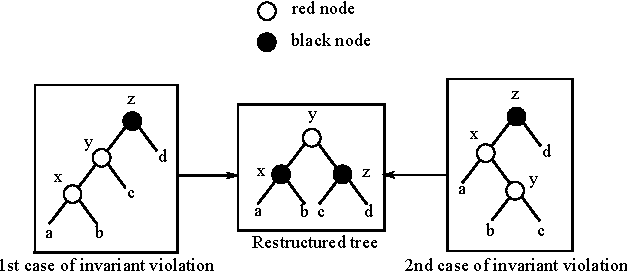
\includegraphics{balancing}
\vspace{5pt}
\caption{Possible cases of 3rd invariant violation after insertion in the left branch of the node.}
\label{fig:balancing}
\end{figure}

\prettyref{fig:balancing} shows 2 possible cases when the 3rd invariant is violated after insertion in the left branch of the node. To repair this invariant the tree must be restructured as shown on the figure. The following code uses pattern matching to implement the restructuring, otherwise the function returns the sub-tree as is:

\begin{Verbatim}
leftBalance :: Node a -> Node a
leftBalance (N B (N R (N R a x b) y c) z d) =
    N R (N B a x b) y (N B c z d)
leftBalance (N B (N R a x (N R b y c)) z d) =
    N R (N B a x b) y (N B c z d)
leftBalance n = n
\end{Verbatim}

The function \verb|rightBalance| is similar. Complete source code is in Appendix A.

\subsection{Proving that the 4th invariant is maintained by insert}

To show that the 4th invariant is maintained by the insertion operation we need to add black height as a parameter of the \verb|Node| data type.

First we define Peano numbers in same way as before:

\begin{Verbatim}
data Nat = Zero | Succ Nat
\end{Verbatim}

Then we turn Node into a GADT with a black height parameter:

\begin{Verbatim}
data Node a (bh::Nat) where
    E :: Node a 'Zero
    N :: Color -> Node a bh -> a -> Node a bh -> Node a ???
\end{Verbatim}

The leaf node has black height $0$. The definition of internal nodes requires that both children have the same black height. The black height of the node itself must be conditionally incremented based on its color. This is implemented using the following type family which computes the new height based on the color of the node and black height of its children. Both parameters are represented as types (of \verb|Color| and \verb|Nat| kinds correspondingly). This code requires \verb|TypeFamilies| and \verb|DataKinds| extensions.

\begin{Verbatim}
type family   IncBlackHeight (c::Color) (bh::Nat) :: Nat
type instance IncBlackHeight R bh = bh
type instance IncBlackHeight B bh = Succ bh
\end{Verbatim}

Now we see that a color must be passed as a type (for \verb|IncBlackHeight| type family) and as a value (to the value constructor). Similarly as before, we need to use a singleton type as a bridge:

\begin{Verbatim}
data ColorSingleton (c::Color) where
    SR :: ColorSingleton R
    SB :: ColorSingleton B
\end{Verbatim}

The value of this singleton type is passed as a parameter to the node value constructor and the color type is used for type family:

\begin{Verbatim}
data Node a (bh::Nat) where
    E :: Node a 'Zero
    N :: ColorSingleton c -> Node a bh -> a
        -> Node a bh -> Node a (IncBlackHeight c bh)
\end{Verbatim}

After we have added a new parameter for the \verb|Node| data type, it is an error to write:

\begin{Verbatim}
type Tree a = Node a bh
\end{Verbatim}

since normally when creating a new type in Haskell, every type variable that appears on the right-hand side of the definition must also appear on its left-hand side. One solution to this problem is usage of \italic{existential types} (this definition requires extension \verb|RankNTypes|):

\begin{Verbatim}
data Tree a = forall bh. Root (Node a bh)
\end{Verbatim}

It is also possible to do this with a GADT:

\begin{Verbatim}
data Tree a where
    Root :: Node a bh -> Tree a
\end{Verbatim}

The implementation of insertion operation never violates the 4th invariant, so the remaining changes are adjustments of type annotations and so on. Complete source code is in Appendix B.

\subsection{Proving that the 3rd invariant is maintained by insert}

Proving the 3rd invariant is more involved. First, we need to specify valid colors for a node on the type level. This can be done using type families as before or using type classes. We choose the latter and define a type class with 3 parameters corresponding to color of the parent and colors of the child nodes (this code requires \verb|MultiParamTypeClasses| extension):

\begin{Verbatim}
class ValidColors (parent::Color) (child1::Color) (child2::Color)
\end{Verbatim}

We do not need to define any functions in this type class, because our aim is just to declare instances with valid colors (this code requires \verb|FlexibleInstances| extension):

\begin{Verbatim}
instance ValidColors R B B
instance ValidColors B c1 c2
\end{Verbatim}

The allowed nodes are:

\begin{itemize}
\item red nodes with black child nodes;
\item black nodes with child nodes of any color.
\end{itemize}

We need to add color type as a parameter to the \verb|Node| data type and restrict it to have only correctly-colored nodes using the \verb|ValidColors| type class:

\begin{Verbatim}
data Node a (bh::Nat) (c::Color) where
    E :: Node a 'Zero B
    N :: ValidColors c c1 c1 => ColorSingleton c -> Node a bh c1
        -> a -> Node a bh c2 -> Node a (IncBlackHeight c bh) c
\end{Verbatim}

With this change we also statically ensure the 2nd invariant: leaf nodes have black color.

We also need to update the definition of the \verb|Tree| data type to specify that root node has black color (this way also ensuring the 1st invariant):

\begin{Verbatim}
data Tree a where
    Root :: Node a bh B -> Tree a
\end{Verbatim}

The implementation of the insertion operation can temporarily invalidate the 3rd invariant (see \prettyref{fig:balancing}), so during insertion we are not able to represent the tree using this data type. Thus, we need to declare a data type similar to \verb|Node|, but without the restriction on node colors:

\begin{Verbatim}
data IntNode a (n::Nat) where
    IntNode :: ColorSingleton c -> Node a n c1 -> a
        -> Node a n c2 -> IntNode a (IncBlackHeight c n)
\end{Verbatim}

As before, we need to make changes in type annotations of the functions implementing insert operation. We also need to change the \verb|leftBalance| function type signature this way:

\begin{Verbatim}
leftBalance :: ColorSingleton c -> IntNode a n -> a
    -> Node a n c' -> IntNode a (IncBlackHeight c n)
\end{Verbatim}

Earlier, we passed the whole node as a parameter. But we can't do this after the \verb|Node| data type was modified: the 3rd invariant could be violated due to insertion in the left branch of the node. So, we pass all parameters of the parameters of the node and left child is represented using \verb|IntNode| data type.

Previous cases should be rewritten using new types:

\begin{Verbatim}
leftBalance SB (IntNode SR (N SR a x b) y c) z d =
    IntNode SR (N SB a x b) y (N SB c z d)
leftBalance SB (IntNode SR a x (N SR b y c)) z d =
    IntNode SR (N SB a x b) y (N SB c z d)
\end{Verbatim}

However, now we can't write the same catch-all case as before:

\begin{Verbatim}
leftBalance c (IntNode c1 a x b) d n2 =
    IntNode c (N c1 a x b) d n2
\end{Verbatim}

This case does not type-check with the following error:

\begin{Verbatim}
Could not deduce (ValidColors c1 c2 c2) ...
\end{Verbatim}

The reason is that the type of the left node is \verb|IntNode|, so even though we have previously balanced the left sub-tree, technically this is not reflected in the type. We need to explicitly match against the correct cases and reconstruct the node. First, we match against the black nodes where children can have any color:

\begin{Verbatim}
leftBalance c (IntNode SB a x b) z d = IntNode c (N SB a x b) z d
\end{Verbatim}

Red nodes must have black children:

\begin{Verbatim}
leftBalance c (IntNode SR a@(N SB _ _ _) x b@(N SB _ _ _)) z d =
    IntNode c (N SR a x b) z d
leftBalance c (IntNode SR E x E) z d = IntNode c (N SR E x E) z d
\end{Verbatim}

Unfortunately, we haven't yet listed all cases. We know that the following cases can't happen, but we do not have enough information in the type to omit them. We can skip them, but this means producing ``Non-exhaustive patterns'' exception for these impossible cases. To workaround the corresponding warning message from Haskell compiler we are using the \verb|error| function:

\begin{Verbatim}
leftBalance _ (IntNode SR (N SR _ _ _) _ _) _ _ =
    error "can't happen"
leftBalance _ (IntNode SR _ _ (N SR _ _ _)) _ _ =
    error "can't happen"
\end{Verbatim}

However, the previous code illustrates a general problem with proofs. In fact, in Haskell $\bot$ (bottom) is a member of every type. As a result, we can write:

\begin{Verbatim}
concatenate :: List a m -> List a n -> List a (Plus m n)
concatenate = undefined
\end{Verbatim}

This code type checks, but, of course, the implementation of the \verb|concatenate| function does not meet our expectations.

At this point, we have specified all cases of the \verb|leftBalance| function (note that the case of one regular node and one leaf node is not valid, because these nodes must have different black heights; so, we do not need to take care of this case). The complete source code of this example is in Appendix C.

To sum up, we have implemented and verified the insertion operation on red-black trees. By using GADTs to express invariants for this data type, we guarantee that the tree is balanced and that searching in such tree will take $O (\log n)$ time (where $n$ is total number of elements in the tree).

\section{Type Signatures for Functions Involving GADTs}
\label{sec:type_signatures}

Type inference for programs with GADTs is out of scope for this article. But when writing programs we are faced with a problem: typically Haskell functions do not require writing type signatures, but many functions involving GADTs do not compile without specifying type signatures explicitly, as the Haskell compiler can not automatically infer the type. This section describes the reasons of this situation.

Hindley-Milner (HM) is the classic type inference method~\cite{cardelli_typechecking}. One of the most important properties of HM is ability to always deduce the \italic{most general type} (\italic{principle type}) of every term.

However, GADTs pose a difficult problem for type inference, because programs with GADTs lose principle type property~\cite{type_inference_gadts}. For example, consider the following GADT program:

\begin{Verbatim}
data Test t where
    TInt :: Int -> Test Int
    TString :: String -> Test String

f (TString s) = s
\end{Verbatim}

There are two possible principal types of the function \verb|f|, but neither of them is an instance of the other:

\begin{Verbatim}
f :: Test t -> String
f :: Test t -> t
\end{Verbatim}

Also without type signature the following function fails to typecheck:

\begin{Verbatim}
f' (TString s) = s
f' (TInt i) = i
\end{Verbatim}

Adding type signature fixes the problem:

\begin{Verbatim}
f' :: Test t -> t
\end{Verbatim}

The paper by Schrijvers et al.~\cite{type_inference_gadts} provides more information on type inference for programs with GADTs.

\section{Usage of GADTs in Yampa}
\label{sec:yampa}

Yampa~\cite{yampa} is a domain-specific language for functional reactive programming (FRP). FRP is a programming paradigm which involves expressing data flows using functional programming languages. Based on the information from the paper by Nilsson~\cite{yampa_gadts}, this section describes how GADTs were used to improve performance of Yampa programs.

The signal function is a central abstraction in Yampa. It represents a simple synchronous process that maps an input signal to an output signal (see \prettyref{fig:signal_function}). The type of the signal function is \verb|SF a b| and it can be constructed from an ordinary function using the following function:

\begin{Verbatim}
arr :: (a -> b) -> SF a b
\end{Verbatim}

\begin{figure}
\centering

\includegraphics{signal_function}
\vspace{5pt}
\caption{Signal function \texttt{SF a b}.}
\label{fig:signal_function}
\end{figure}

The following function provides a composition of signal functions (as shown in \prettyref{fig:signal_composition}):

\begin{Verbatim}
(>>>) :: SF a b -> SF b c -> SF a c
\end{Verbatim}

\begin{figure}
\centering
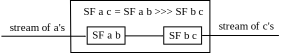
\includegraphics{signal_composition}
\caption{Composition of signal functions.}
\label{fig:signal_composition}
\vspace{5pt}
\end{figure}

There is a natural requirement to eliminate the overhead of composition with identity function:

\begin{Verbatim}
arr id >>> f = f
f >>> arr id = f
\end{Verbatim}

As an attempt to implement this in Yampa we can imagine introducing a special value constructor to represent identity signal functions:

\begin{Verbatim}
data SF a b = ...
            | SFId -- Represents arr id.
\end{Verbatim}

But the return type of this value constructor is still \verb|SF a b|. We can use the same trick as before with phantom types. We can define a function to construct the value and restrict the type to \verb|SF a a|:

\begin{Verbatim}
identity :: SF a a
identity = SFId
\end{Verbatim}

Now we can try to use the new value constructor in the definition of the function \verb|>|\verb|>|\verb|>| this way:

\begin{Verbatim}
(>>>) :: SF a b -> SF b c -> SF a c
...
SFId >>> sf = sf
sf >>> SFId = sf
\end{Verbatim}

But this code does not type check, because when we pattern match using \verb|SFId| value constructor, the type is still \verb|SF a b|, not \verb|SF a a|. We have already seen this problem before when we attempted to use phantom types for expression evaluation. The solution is to use GADT to represent the signal function:

\begin{Verbatim}
data SF a b where
    ...
    SFId :: SF a a
\end{Verbatim}

After this change the function \verb|>|\verb|>|\verb|>| as presented above must type check due to type refinement in pattern matching.

\begin{table}[float,captionpos=b,belowcaptionskip=4pt]
\centering
\begin{tabular}{cll}
\hline\noalign{\smallskip}
Benchmark & $T_S$[s] & $T_G$[s]\\
\noalign{\smallskip}
\hline
\noalign{\smallskip}
1 & 0.41 & 0.00 \\
2 & 0.74 & 0.22 \\
3 & 0.45 & 0.22 \\
4 & 1.29 & 0.07 \\
5 & 1.95 & 0.08 \\
6 & 1.48 & 0.69 \\
7 & 2.85 & 0.72 \\
\hline
\end{tabular}
\label{tab:yampa_performance}
\caption{Performance improvements enabled by GADTs in Yampa programs}
\end{table}

There are other performance improvements that are enabled by GADTs in Yampa~\cite{yampa_gadts}. The results of performance improvements described by the paper by Nilsson~\cite{yampa_gadts} are shown in the table. The table shows execution time of several benchmarks using initial simply-optimized implementation ($T_S$) and the implementation with GADT-based optimizations ($T_G$). In addition to performance improvements, GADTs allowed the authors of the paper to write a more concise and cleaner API without the need of pre-composed signal functions (which were defined in Yampa only for performance reasons).

\section{GADTless Programming}
\label{sec:gadtless}

Previous sections should convince the reader that GADTs are a very powerful and helpful extension of the language. However, there are cases when this extension is not available (for example, this feature is not implemented in Hugs compiler). For this reason, there is an interest in replacing them with simpler features while not substantially changing programs and their meanings. This is called GADTless programming~\cite{gadtless}.

Earlier we discussed implementation of expression evaluator using GADT. It can also be implemented using type classes~\cite{finally_tagless}:

\begin{Verbatim}
class Expr e where
    intVal  :: Int -> e Int
    boolVal :: Bool -> e Bool
    add     :: e Int -> e Int -> e Int
    isZero  :: e Int -> e Bool
    if'     :: e Bool -> e t -> e t -> e t
\end{Verbatim}

Bad expressions are still rejected by the type checker:

\begin{Verbatim}
ghci> :t isZero $ boolVal True
Couldn't match expected type `Int' with actual type `Bool'...
ghci> :t isZero $ intVal 5
isZero $ intVal 5 :: Expr e => e Bool
\end{Verbatim}

Evaluation is implemented by defining a helper data type as an instance of \verb|Expr e| type class:

\begin{Verbatim}
newtype Eval a = Eval {runEval :: a}

instance Expr Eval where
    intVal x  = Eval x
    boolVal x = Eval x
    add x y   = Eval $ runEval x + runEval y
    isZero x  = Eval $ runEval x == 0
    if' x y z = if (runEval x) then y else z 

t = runEval $ isZero $ intVal 5
\end{Verbatim}

Printing expressions is implemented in a similar way:

\begin{Verbatim}
newtype Print a = Print {printExpr :: String}

instance Expr Print where
    intVal x  = Print $ show x
    boolVal x = Print $ show x
    add x y   = Print $ printExpr x ++ "+" ++ printExpr y
    isZero x  = Print $ "isZero(" ++ printExpr x ++ ")"
    if' x y z = Print $ "if (" ++ printExpr x ++ ") then (" ++
        printExpr y ++ ") else (" ++ printExpr z ++ ")"

t' = printExpr $ isZero $ intVal 5
\end{Verbatim}

Detailed discussion of GADTless programming and comparing advantages of these approaches is out of scope of this paper. However, it is worth pointing out that it is much easier to do deep pattern matching with data types (including GADTs) than with class instances. For example, earlier we have used deep pattern matching in \verb|leftBalance| function:

\begin{Verbatim}
leftBalance :: Node a -> Node a
leftBalance (N B (N R (N R a x b) y c) z d) =
    N R (N B a x b) y (N B c z d)
leftBalance (N B (N R a x (N R b y c)) z d) =
    N R (N B a x b) y (N B c z d)
leftBalance n = n
\end{Verbatim}

Another important aspect is that GADTs, just like all data types in Haskell, are closed: once they are declared, they can not be extended in the rest of the program. This issue is called the \italic{expression problem}~\cite{expression_problem}. Wouter Swierstra describes a technique to solve this problem in the article ``Data types \`{a} la carte''~\cite{a_la_carte}.

In contrast, type class instances are open. For example, we could split \verb|Expr e| type class into two separate type classes (this way we improve modularity):

\begin{Verbatim}
class ArithExpr e where
    intVal  :: Int -> e Int
    add     :: e Int -> e Int -> e Int
    isZero  :: e Int -> e Bool

class LogExpr e where
    boolVal :: Bool -> e Bool
    if'     :: e Bool -> e t -> e t -> e t
    
class (ArithExpr e, LogExpr e) => Expr e
\end{Verbatim}

\section{Conclusion}
\label{sec:conclusion}

This article has demonstrated the use of GADTs in practice:

\begin{longitem}
\item We have shown that GADTs are useful for domain-specific embedded languages: they allow to statically type-check valid expressions.
\item GADTs allow to express datatype-generic functions using representation types and universal data types.
\item GADTs can be used as a lightweight way to ensure program correctness. They allow to encode domain-specific invariants in data type. The programmer can decide which parts of her or his program require verification and add only relevant invariants. Haskell enforces a phase separation between run-time values and compile-time types. Invariants are expressed using types, so there is no additional run-time cost. But on the other hand, we have shown the issue with the $\bot$ value.
\item We have also described how GADTs were used to improve performance of Yampa programs.
\end{longitem}

\section*{Acknowledgments}

This tutorial article was inspired by Simon Peyton-Jones talk at LASER 2012 summer school. The source code for the red-black tree example was originally written by Stephanie Weirich for a university course. The author is thankful to have ability to use this great example of GADTs usage in this tutorial. Also the author would like to thank Simon Peyton-Jones, Owen Stephens, Alexander Batischev, Denis Kasak, Mann mit Hut, Alexei Alexandrov, Serge Le Huitouze, Eric Mullen, Egor Kazachkov and Vadim Zaytsev for the review of the article draft and providing valuable comments.

\bibliography{gadt}

\section*{Appendix A. Original Red-Black Tree Source Code}
\label{sec:appendix_a}

\begin{Verbatim}
module RBT1 where

data Color = R | B
data Node a = E | N Color (Node a) a (Node a) 
type Tree a = Node a

member :: Ord a => a -> Tree a -> Bool
member _ E  = False
member x (N _ l a r)
    | x < a  = member x l
    | x > a  = member x r
    | otherwise = True

insert :: Ord a => Tree a -> a -> Tree a
insert t v = blacken (insertInternal t v) where
    insertInternal n@(N c l a r) x
        | x < a = leftBalance  (N c (insertInternal l x) a r)
        | x > a = rightBalance (N c l a (insertInternal r x))
        | otherwise = n
    insertInternal E x = N R E x E
    blacken (N _ l x r) = N B l x r

leftBalance :: Node a -> Node a
leftBalance (N B (N R (N R a x b) y c) z d) =
    N R (N B a x b) y (N B c z d)
leftBalance (N B (N R a x (N R b y c)) z d) =
    N R (N B a x b) y (N B c z d)
leftBalance n = n

rightBalance :: Node a -> Node a
rightBalance (N B a x (N R b y (N R c z d))) =
    N R (N B a x b) y (N B c z d)
rightBalance (N B a x (N R (N R b y c) z d)) =
    N R (N B a x b) y (N B c z d)
rightBalance n = n
\end{Verbatim}

\section*{Appendix B. Red-Black Tree Source Code: Proving the Forth Invariant}
\label{sec:appendix_b}

\begin{Verbatim}
{-# LANGUAGE TypeFamilies, DataKinds, GADTs #-}

module RBT2 where

data Color = R | B
data ColorSingleton (c::Color) where
    SR :: ColorSingleton R
    SB :: ColorSingleton B

data Nat = Zero | Succ Nat

type family   IncBlackHeight (c::Color) (bh::Nat) :: Nat
type instance IncBlackHeight R bh = bh
type instance IncBlackHeight B bh = Succ bh

data Node a (bh::Nat) where
    E :: Node a 'Zero
    N :: ColorSingleton c -> Node a bh -> a
        -> Node a bh -> Node a (IncBlackHeight c bh)

data Tree a where
    Root :: Node a bh -> Tree a

insert :: Ord a => Tree a -> a -> Tree a
insert (Root t) v = blacken (insertInternal t v) where
    insertInternal :: Ord a => Node a n -> a -> Node a n
    insertInternal n@(N c l a r) x
        | x < a = leftBalance  (N c (insertInternal l x) a r)
        | x > a = rightBalance (N c l a (insertInternal r x))
        | otherwise = n
    insertInternal E x = N SR E x E
    blacken (N _ l x r) = Root (N SB l x r)

leftBalance :: Node a bh -> Node a bh
leftBalance (N SB (N SR (N SR a x b) y c) z d) =
    N SR (N SB a x b) y (N SB c z d)
leftBalance (N SB (N SR a x (N SR b y c)) z d) =
    N SR (N SB a x b) y (N SB c z d)
leftBalance n = n

rightBalance :: Node a bh -> Node a bh
rightBalance (N SB a x (N SR b y (N SR c z d))) =
    N SR (N SB a x b) y (N SB c z d)
rightBalance (N SB a x (N SR (N SR b y c) z d)) =
    N SR (N SB a x b) y (N SB c z d)
rightBalance n = n
\end{Verbatim}

\section*{Appendix C. Red-Black Tree Source Code: Proving the Third Invariant}
\label{sec:appendix_c}

\begin{Verbatim}
{-# LANGUAGE TypeFamilies, DataKinds, GADTs, RankNTypes #-}
{-# LANGUAGE MultiParamTypeClasses, FlexibleInstances #-}

module RBT3 where

data Color = R | B
data ColorSingleton (c::Color) where
    SR :: ColorSingleton R
    SB :: ColorSingleton B

data Nat = Zero | Succ Nat

type family   IncBlackHeight (c::Color) (bh::Nat) :: Nat
type instance IncBlackHeight R bh = bh
type instance IncBlackHeight B bh = Succ bh

class ValidColors (parent::Color) (child1::Color) (child2::Color)
instance ValidColors R B B
instance ValidColors B c1 c2

data Node a (bh::Nat) (c::Color) where
    E :: Node a 'Zero B
    N :: ValidColors c c1 c1 => ColorSingleton c -> Node a bh c1
        -> a -> Node a bh c2 -> Node a (IncBlackHeight c bh) c

data Tree a where
    Root :: Node a bh B -> Tree a

data IntNode a (n::Nat) where
    IntNode :: ColorSingleton c -> Node a n c1 -> a
        -> Node a n c2 -> IntNode a (IncBlackHeight c n)
\end{Verbatim}

\begin{Verbatim}
insert :: Ord a => Tree a -> a -> Tree a
insert (Root t) v = blacken (insertInternal t v) where
    insertInternal :: Ord a => Node a n c -> a -> IntNode a n
    insertInternal (N c l a r) x
        | x < a = leftBalance  c (insertInternal l x) a r
        | x > a = rightBalance c l a (insertInternal r x)
        | otherwise = IntNode c l a r
    insertInternal E x = IntNode SR E x E
    blacken (IntNode _ l x r) = Root (N SB l x r)

leftBalance :: ColorSingleton c -> IntNode a n -> a
    -> Node a n c' -> IntNode a (IncBlackHeight c n)
leftBalance SB (IntNode SR (N SR a x b) y c) z d =
    IntNode SR (N SB a x b) y (N SB c z d)
leftBalance SB (IntNode SR a x (N SR b y c)) z d =
    IntNode SR (N SB a x b) y (N SB c z d)
leftBalance c (IntNode SB a x b) z d = IntNode c (N SB a x b) z d
leftBalance c (IntNode SR a@(N SB _ _ _) x b@(N SB _ _ _)) z d =
    IntNode c (N SR a x b) z d
leftBalance c (IntNode SR E x E) z d = IntNode c (N SR E x E) z d
leftBalance _ (IntNode SR (N SR _ _ _) _ _) _ _ =
    error "can't happen"
leftBalance _ (IntNode SR _ _ (N SR _ _ _)) _ _ =
    error "can't happen"

rightBalance :: ColorSingleton c -> Node a n c' -> a
    -> IntNode a n -> IntNode a (IncBlackHeight c n)
rightBalance SB a x (IntNode SR b y (N SR c z d)) =
    IntNode SR (N SB a x b) y (N SB c z d)
rightBalance SB a x (IntNode SR (N SR b y c) z d) =
    IntNode SR (N SB a x b) y (N SB c z d)
rightBalance c a x (IntNode SB b y d) = IntNode c a x (N SB b y d)
rightBalance c a x (IntNode SR b@(N SB _ _ _) y d@(N SB _ _ _)) =
    IntNode c a x (N SR b y d)
rightBalance c a x (IntNode SR E y E) = IntNode c a x (N SR E y E)
rightBalance _ _ _ (IntNode SR (N SR _ _ _) _ _) =
    error "can't happen"
rightBalance _ _ _ (IntNode SR _ _ (N SR _ _ _)) =
    error "can't happen"
\end{Verbatim}

\end{document}






































